%!TEX root = ../../csuthesis_main.tex
\chapter{绪论}



\section{研究背景}

随着人工智能和计算机视觉技术的飞速发展,自动驾驶逐渐成为交通运输领域的核心研究方向。车辆需要通过视觉感知系统实时获取周围环境信息,包括行人、车辆、交通信号灯及障碍物等,以为路径规划和车辆控制提供支持。目标检测与目标跟踪作为环境感知的重要组成部分,不仅需要高效识别目标的位置,还需结合目标轨迹与运动趋势进行深入分析,尤其是在复杂交通场景下对潜在危险的判断更为关键。

近年来,YOLO(You Only Look Once)系列目标检测算法凭借高效的实时性能,成为自动驾驶领域广泛采用的技术。然而,在动态交通环境中,单纯的目标检测无法满足对目标行为的全面理解和预测需求。因此,将目标跟踪与意图分析结合,通过运动趋势和行为预测进一步增强系统的决策能力,是当前研究的热点方向。

在目标跟踪中,DeepSORT等算法能够通过轨迹关联和状态估计,实时获取目标的位置、速度和运动方向,为行为意图的推断提供基础。在意图分析中,基于相对速度和轨迹趋势的计算,可以有效判断目标是否接近或远离本车,并结合时间到碰撞(Time-to-Collision, TTC)等指标量化潜在风险。此外,卡尔曼滤波、交互多模型(IMM)滤波器等经典方法在轨迹预测中表现出稳定性,而深度学习模型如LSTM、Transformer在复杂场景下具有更高的预测精度。

本文基于YOLO目标检测算法,结合多目标跟踪与意图分析,提出一种适用于自动驾驶场景的综合解决方案。通过实时检测和跟踪动态目标,并分析其运动趋势和潜在意图,为自动驾驶车辆的安全决策和路径优化提供有力支持。

\section{研究意义}

\subsection{理论意义}

基于YOLO目标检测的多目标跟踪与意图分析研究,将进一步深化深度学习技术在自动驾驶环境感知中的应用。通过结合目标检测、轨迹预测和意图分析,为目标行为预测提供新的理论框架和技术支撑。本研究将丰富计算机视觉领域中目标检测与跟踪的研究方法,尤其是将运动趋势和潜在危险分析纳入系统建模,为复杂动态场景下的多目标行为分析提供创新的解决方案。此外,通过引入高效的意图分析算法,推动自动驾驶车辆对潜在风险的准确识别和预测能力的优化,从而提高自动驾驶技术在实际场景中的适用性和可靠性。

\subsection{现实意义}

自动驾驶车辆在实际道路中面临多变且动态的环境,传统的单一目标检测方法难以满足复杂场景中的风险评估需求。本研究提出的多目标跟踪与意图分析算法,能够实时获取动态目标的位置、速度和运动趋势,并预测其潜在行为,有效增强自动驾驶车辆对危险的感知和应对能力。通过这一研究,自动驾驶车辆可以更早地识别潜在风险并作出安全决策,从而减少交通事故,提升道路安全性。同时,这一研究将推动自动驾驶技术的工程化应用,为实现更智能、更安全的无人驾驶提供重要技术支持。
当前的自动驾驶系统中,虽然有目标检测和跟踪的研究,但大多数研究侧重于单一任务,例如目标的实时检测或跟踪,缺乏对目标意图(如接近、远离、本车行为等)的综合分析。现有方法大多没有考虑如何将跟踪结果与目标行为预测相结合来提升决策质量。
本文的研究可以结合YOLO目标检测与深度学习的多目标跟踪算法,如DeepSORT,进一步将目标的运动轨迹与行为意图进行融合,从而提供一个全面的系统,既能实时检测和跟踪多目标,又能分析目标的意图(如是否接近本车、是否存在潜在碰撞等),填补目前在目标跟踪与意图分析综合算法方面的空白。

\section{国内外研究现状}

\subsection{目标检测研究现状}

目标检测是指将图像或者视频中的目标与其他不感兴趣区域进行区分,判断是否存在目标,以及确定目标位置和识别目标种类的计算机视觉任务。以是否使用深度学习为分界线,可以将目标检测算法分为传统的目标检测算法和基于深度学习的目标检测算法。传统的目标检测算法依赖于人工设计的特征算子,并采用特征提取加分类器的模式来实现。Viola和Jones提出了Viola-Jones人脸检测器 \cite{viola2001rapid},该检测器使用Haar-like特征提取算子,利用Adaboost分类器进行分类,并采用由多个分类器组成的Cascade级联分类器来提高识别率。Navneet Dalal等人\cite{dalal2005histograms}提出方向梯度直方图(Histogram of Oriented Gradients,HOG),HOG是一种用于目标检测的特征描述算子,通过计算图像中局部梯度的方向信息,对图像的浅层外观特征进行提取。由于HOG过度依赖局部梯度信息,因此在复杂场景下的特征提取能力较差。Felzenszwalb等人\cite{felzenszwalb2009object}在HOG的基础上,提出了可变形组件模组(Deformable Part Model,DPM)。DPM采用多组件策略,将目标分解为多个部分后进行建模,因此DPM对目标的形变具有很强的鲁棒性。传统的目标检测算法大多使用人工设置的特征提取算子来对图像进行特征提取,在面对多尺度、密集目标、极端天气等复杂环境时,算法的鲁棒性和准确率都会大大降低。同时采用滑动窗口来对图像特征进行逐一计算的方式,会使算法的计算复杂度过高。因此传统的目标检测方法无法满足实时检测需求,不能很好地在工业中进行应用。

随着深度学习的飞速发展,目标检测领域的研究取得了突破性的进展。与传统的目标检测算法相比,基于深度学习的目标检测模型在经过大量图像数据训练后,能“学会”如何提取目标特征,在面对不同尺度的目标以及复杂场景时,具有更好的鲁棒性和泛化能力。根据是否需要生成候选区域,可以将基于深度学习的目标检测算法分为单阶段(one-stage)与两阶段(two-stage)。两阶段的目标检测算法主要分为两步,首先筛选出图片中可能包含物体的候选区域,接着再对候选区域中的特征进行分类回归。Ross Girshick等人\cite{girshick2014rich}提出R-CNN目标检测算法,首先对输入图像使用选择搜索\cite{uijlings2013selective}(selective search)网络获得大约2000个不同尺度的候选区域,接着对所有的候选区域进行统一缩放,将尺寸变为227×227。再通过卷积神经网络(Convolutional Neural Networks,CNN)对所有候选区域中的特征进行提取,得到维度为2000×4096的特征向量。最后再利用SVM分类器对特征向量进行分类,以及使用回归器来对边界框的位置进行调整。由于R-CNN目标检测算法需要对约2000个候选框逐一进行特征提取,而候选框之间又存在许多包含相同特征的区域,这就导致整个过程中存在大量冗余操作,严重影响了检测速度。为了解决上述问题,Ross Girshick等人\cite{girshick2015fast}又提出了Fast R-CNN,Fast R-CNN首先对输入的图像进行卷积,得到对应的特征图。接着将事先处理好的区域候选框投影到特征图上。采用这种方式只需要进行一次卷积,可以减少大量冗余的卷积计算。而且与R-CNN所使用的分类任务+回归任务模式不同,Fast R-CNN将二者融合在一个网络中,不再需要对分类器和回归器进行单独训练。但是Fast R-CNN算法依然沿用了使用选择搜索算法的方式来获取候选区域,该过程不仅操作耗时而且容易漏掉包含目标的区域。因此Shaoqing Ren等人\cite{ren2015faster}又提出了Faster R-CNN,算法采用区域建议网络(Region Proposal Networks,RPN)来获取区域候选框,实现了生成候选区域过程与目标检测任务的融合。同时Faster R-CNN还提出了锚框(Anchor)这一重要思想,锚框是指在图像上预先设置好多组尺寸比例不同的参照框,来尽可能地包含物体出现的位置。He Kaiming\cite{he2017mask}等人在Faster R-CNN的基础上提出了Mask R-CNN,该算法使用ROIAlign替换Faster R-CNN中的ROIPooling。ROIAlign可以将任意尺寸感兴趣区域的特征图划分为具有固定尺寸的小特征图,并使用双线性插值取代了ROIPooling中的直接取整操作,解决了ROIPooling操作中因两次量化造成的区域不匹配(mis-alignment)问题。在目标检测任务中,使用IOU阈值来区分正负样本。当IOU阈值越大,正样本的数量就会减少,而减小IOU阈值又会学习到大量无关特征。Cai等人cite{cai2018cascade}为了解决上述问题,提出了Cascade R-CNN,该算法采用级联式的结构,通过对多个感知器使用递增的IOU阈值进行训练,来解决因提高IOU阈值所引起的模型过拟合问题。

\subsection{目标跟踪研究现状}

多目标跟踪算法可以分为基于检测跟踪(Tracking by Detection, TBD)和联合检测跟踪(Joint Detecting Tracking, JDT)两种方式。TBD 目标跟踪算法是指先使用目标检测算法得到包含物体的边界框,接着再获取目标的运动信息和外观信息等,最后通过数据关联算法来计算目标间的亲和力并关联目标。Bewley等人\cite{bewley2016simple}提出了 SORT 算法,作为经典的基于检测的目标跟踪算法,采用 Faster R-CNN 作为检测器,利用卡尔曼滤波来预测和更新物体的运动特征信息,通过匈牙利算法进行数据关联,以及使用 IOU 作为度量指标来建立关系,从而实现对多目标进行追踪。Wojke 等人\cite{wojke2017simple}提出了 DeepSORT 多目标跟踪算法,该算法在 SORT 的基础上加入级联匹配,引入了卷积神经网络来提取目标外观特征,有效地减少了在面对遮挡情况下发生身份切换的问题。Yu 等人\cite{yu2016poi}提出了 POI 算法,采用 Faster R-CNN 作为检测器,并使用 skip pooling 和 multi-region 两种策略来提高检测精度,利用改进的 GoogLeNet\cite{szegedy2015going}网络进行特征提取。Sun 等人\cite{sun2019deep}提出了深度亲和网络(DAN),DAN 网络以端到端的方式对目标物体的外观特征进行学习,通过物体和环境的分层特征计算出在不同帧中目标之间的亲和度。Chen 等人\cite{chen2018real}将检测和跟踪结果组成一对候选框,提出了一种得分函数用于衡量每一对候选框的匹配程度,使用非极大值抑制算法依据得分情况进行筛选。Zhang 等人\cite{zhang2021fairmot}将目标检测任务和特征提取融合到一个网络中完成。首先使用编码器-解码器模块对图像进行特征提取,在进行分流后,使用两个分支分别进行边界框预测以及目标外观特征提取,最后使用预测目标中心点处的特征进行边界框时序联结。Liang 等人\cite{liang2022rethinking}提出 CSTrack 算法,采用 CCN(交叉相关网络)来改进检测与重识别间的协作学习。将目标检测和外观特征提取进行解耦,通过使用自注意力的方式获得自注意力权重图和交叉相关性权重图,并利用 SAAN\cite{zhao2020saan}(尺度感知注意力网络)对特征提取网络进行优化。Liang 等人\cite{liang2022fake}在 CSTrack 的基础上引入时间信息来修正检测器结果,并提出了重检测网络来重新加载被错误分类的目标。Yu 等人\cite{yu2022relationtrack}提出了 GCD(Global Context Disentangling)模块,该模块能将特征图解耦成检测特征和重识别特征两部分,同时采用可变形注意力机制来学习目标和环境之间的关系。

联合检测跟踪算法是将检测任务与跟踪任务进行合并,仅使用一个网络来实现多目标跟踪任务。Peng 等人\cite{peng2020chained}提出了一种 CTracker 算法,该算法首次将目标检测、特征提取、数据关联三个模块集成到单个网络中,实现了端到端的联合检测跟踪。同时还设计了一种联合注意力模块(JAM,Joint Attention Module)来突出检测框中的有效信息区域。Xu 等人\cite{xu2020deep}提出了 DHN(深度匈牙利算法),以可微的方式对检测框和预测框进行匹配,以及提出了一种新的损失函数用于训练联合检测跟踪范式的多目标跟踪器。Pang 等人\cite{pang2021quasidense}提出 QDTrack 算法,通过采用多个正负样本同时计算损失的方式来对特征提取网络进行训练,是一种只利用 ReID 特征而不需要位置和运动信息的多目标跟踪方法。Zhou 等人\cite{zhou2020tracking}提出了 CenterTrack 算法,使用 CenterNet\cite{zhou2019objects}目标检测算法来对目标中心进行定位,CenterTrack 依据上一帧的检测结果得到热量图,峰值代表目标中心点,并采用高斯渲染的方法进行模糊处理。模型利用两个额外的并行分支来预测当前目标相对于上一帧时的水平和竖直方向偏移量。Wu 等人\cite{wu2021track}提出了一种在线多目标联合检测追踪模型,使用 CenterNet 提取图像特征,利用 CVA 模块计算两帧图像中目标的偏移量,得到目标之间的关联性,通过 MFW 模块来传播和增强目标特征,最后使用头部网络将传播特征和当前特征进行处理以实现检测和追踪。Wang 等人\cite{wang2021multiple}提出了 CorrTracker 算法,利用局部相关模块来构建目标与周围环境之间的拓扑关系,从而加强模型在密集场景中的识别能力。Sun 等人\cite{sun2020transtrack}提出 TransTrack 算法,该算法采用 transformer\cite{vaswani2017attention}架构,利用 Query-Key 机制来跟踪当前帧中已存在的目标以及对新目标进行检测。通过在一次拍摄中完成目标检测和目标关联,建立了一种新的联合检测跟踪范式。Chu 等人\cite{chu2023transmot}提出了 STGT 模型,通过将追踪目标轨迹视作稀疏赋权图来构建目标间的空间关系。STGT 构建了一个空间图 transformer 编码器、时间 transformer 编码器和一个空间 transformer 解码器。利用稀疏图来提升训练和推理时的计算速度。并且由于获取了目标间的结构信息,因此比一般的 transformer 也更加有效。

\subsection{意图分析研究现状}

  最早关于识别驾驶意图的讨论可以追溯到 Andrew 等人的一项研究\cite{liu1997realtime},他们认为可以通过分析驾驶员的行为动作来预测其意图,并在研究中仅使用车辆的动态数据,例如横摆角、横摆角速度和车速,来判断驾驶员是否有转弯或换道的意图。要对周围车辆的换道意图进行识别,需要结合感知、数据融合、数据处理等多种技术\cite{zhang2023highway}。感知与数据融合技术融合所有从传感设备传输的信号,生成周围所有交通和其他环境的信息。智能车辆将这些信息从自身的车辆坐标系转换为目标车辆坐标系,并处理为识别算法可以使用的特征变量。因此,在识别方法之外,特征变量的选择对识别的效果也影响重大。针对单个目标车辆,目前广泛使用的信号包括纵向/横向位置、速度和加速度\cite{woo2017lane}。主车的意图识别可以通过车内传感器获得大量有效信息,比如方向盘和制动/油门踏板信号,甚至驾驶员本身的状态等。然而,在车联网技术尚未成熟的当下,目标车辆内的这些信息难以获取。Zhang 等\cite{zhang2018lane}使用目标车辆及其四辆邻近交通车辆的信息,包括它们之间的相对速度和距离,来预测换道行为。Leonhardt 等\cite{leonhardt2017feature}也采用了类似的特征变量来研究换道预测。部分研究使用了目标车辆周围的更多相邻车辆以及与每个相邻车辆相关的更多信息(比如状态量的历史记录)\cite{patel2018predicting}。Altch 等\cite{altche2017lstm}甚至考虑了九辆车来提高预测性能。

  2016 年,日产研制出了前沿科技 ProPILOT,其安装的实力强劲的摄像机可以较为容易的检测出车相对道路的偏离距离\cite{zhang2016nissan}。雪铁龙 LDWS 系统安装有 6 个电子传感器。汽车通过车道标记线的时候,光线的反射不一样,此时检测单元会将信息发送到车载控制中心,内置的振动马达会向驾驶员传递警告信息。这个系统的价格低廉,系统的适应性不错,但是在复杂的电子环境下的表现会受到影响,元器件的精度会降低,目前在 C5、C6 的车型上有应用。Google 也进行了相关研发,利用高性能的软件和智能探测装置,融合雷达和摄像技术,能够在复杂条件下全面的探测周围环境\cite{wang2020autonomous},其结合 GPS 技术的车道偏离技术可以及时矫正汽车的行驶轨迹,并且误差可以达到厘米级。Enache 等\cite{enache2009driver}提出了新的计算方法,通过预瞄偏差及车辆方向偏差综合信息来估计车路之间的相对距离;Cualain 等\cite{cualain2012automotive}利用卡尔曼滤波和霍夫变换建立了车道边界的模型,计算车辆本身的参数及建立新的预警规范来设计预警系统的阈值;Mammar 等cite{mammar2006time}通过计算道路曲率、方向偏差等估计车辆跨过车道线的时间;Ulsoy 等\cite{chiu1996time}利用准确度较高的算法估计TLC 的不确定,考虑到了不同方面的误差;Gaikwad 等\cite{gaikwad2015lane}通过对感兴趣区域的划分,建立实际车道偏离的度量标准。

\subsection{本文结构框架}

本文首先对研究背景及研究意义进行了详细阐述,其中包括本研究在理论层面和实际应用层面的重要性。接着,通过对国内外相关文献的梳理,综合分析了目标识别、目标跟踪和意图分析领域的研究现状,重点关注深度学习技术在这些领域中的方法与应用,明确当前研究的主要成果与存在的不足,为后续研究提供支撑。针对本研究问题所需的关键理论与技术,本文进行了详细分析,包括深度学习的基础理论、YOLO系列目标检测模型、多目标跟踪中的DeepSORT算法,以及轨迹预测与意图分析相关的技术方法。这一部分的内容为算法设计和实验仿真提供了理论依据。

算法设计分为两部分:一是视觉目标检测与多目标跟踪模块,重点描述YOLO与DeepSORT算法的融合与改进;二是基于目标轨迹与速度信息的意图分析模块,使用预训练模型获得目标识别跟踪的结果对象后,对此数据进行处理,用于判断车辆接近或远离的危险程度。

在实验与仿真部分,论文基于Carla仿真平台设计了实验环境。通过构建符合实际交通场景的数据集与仿真场景,对算法的性能进行了全面验证。实验结果从目标检测与跟踪精度、意图分析准确性以及危险评估效果等方面进行了分析与评价,展现了算法的有效性与应用潜力。

最后,论文总结了研究工作,梳理了取得的主要成果,指出了研究中存在的不足,并对未来的研究方向进行了展望,为自动驾驶场景下的视觉目标跟踪与意图分析提供了进一步发展的思路。
\begin{figure}[htbp]
    \centering
    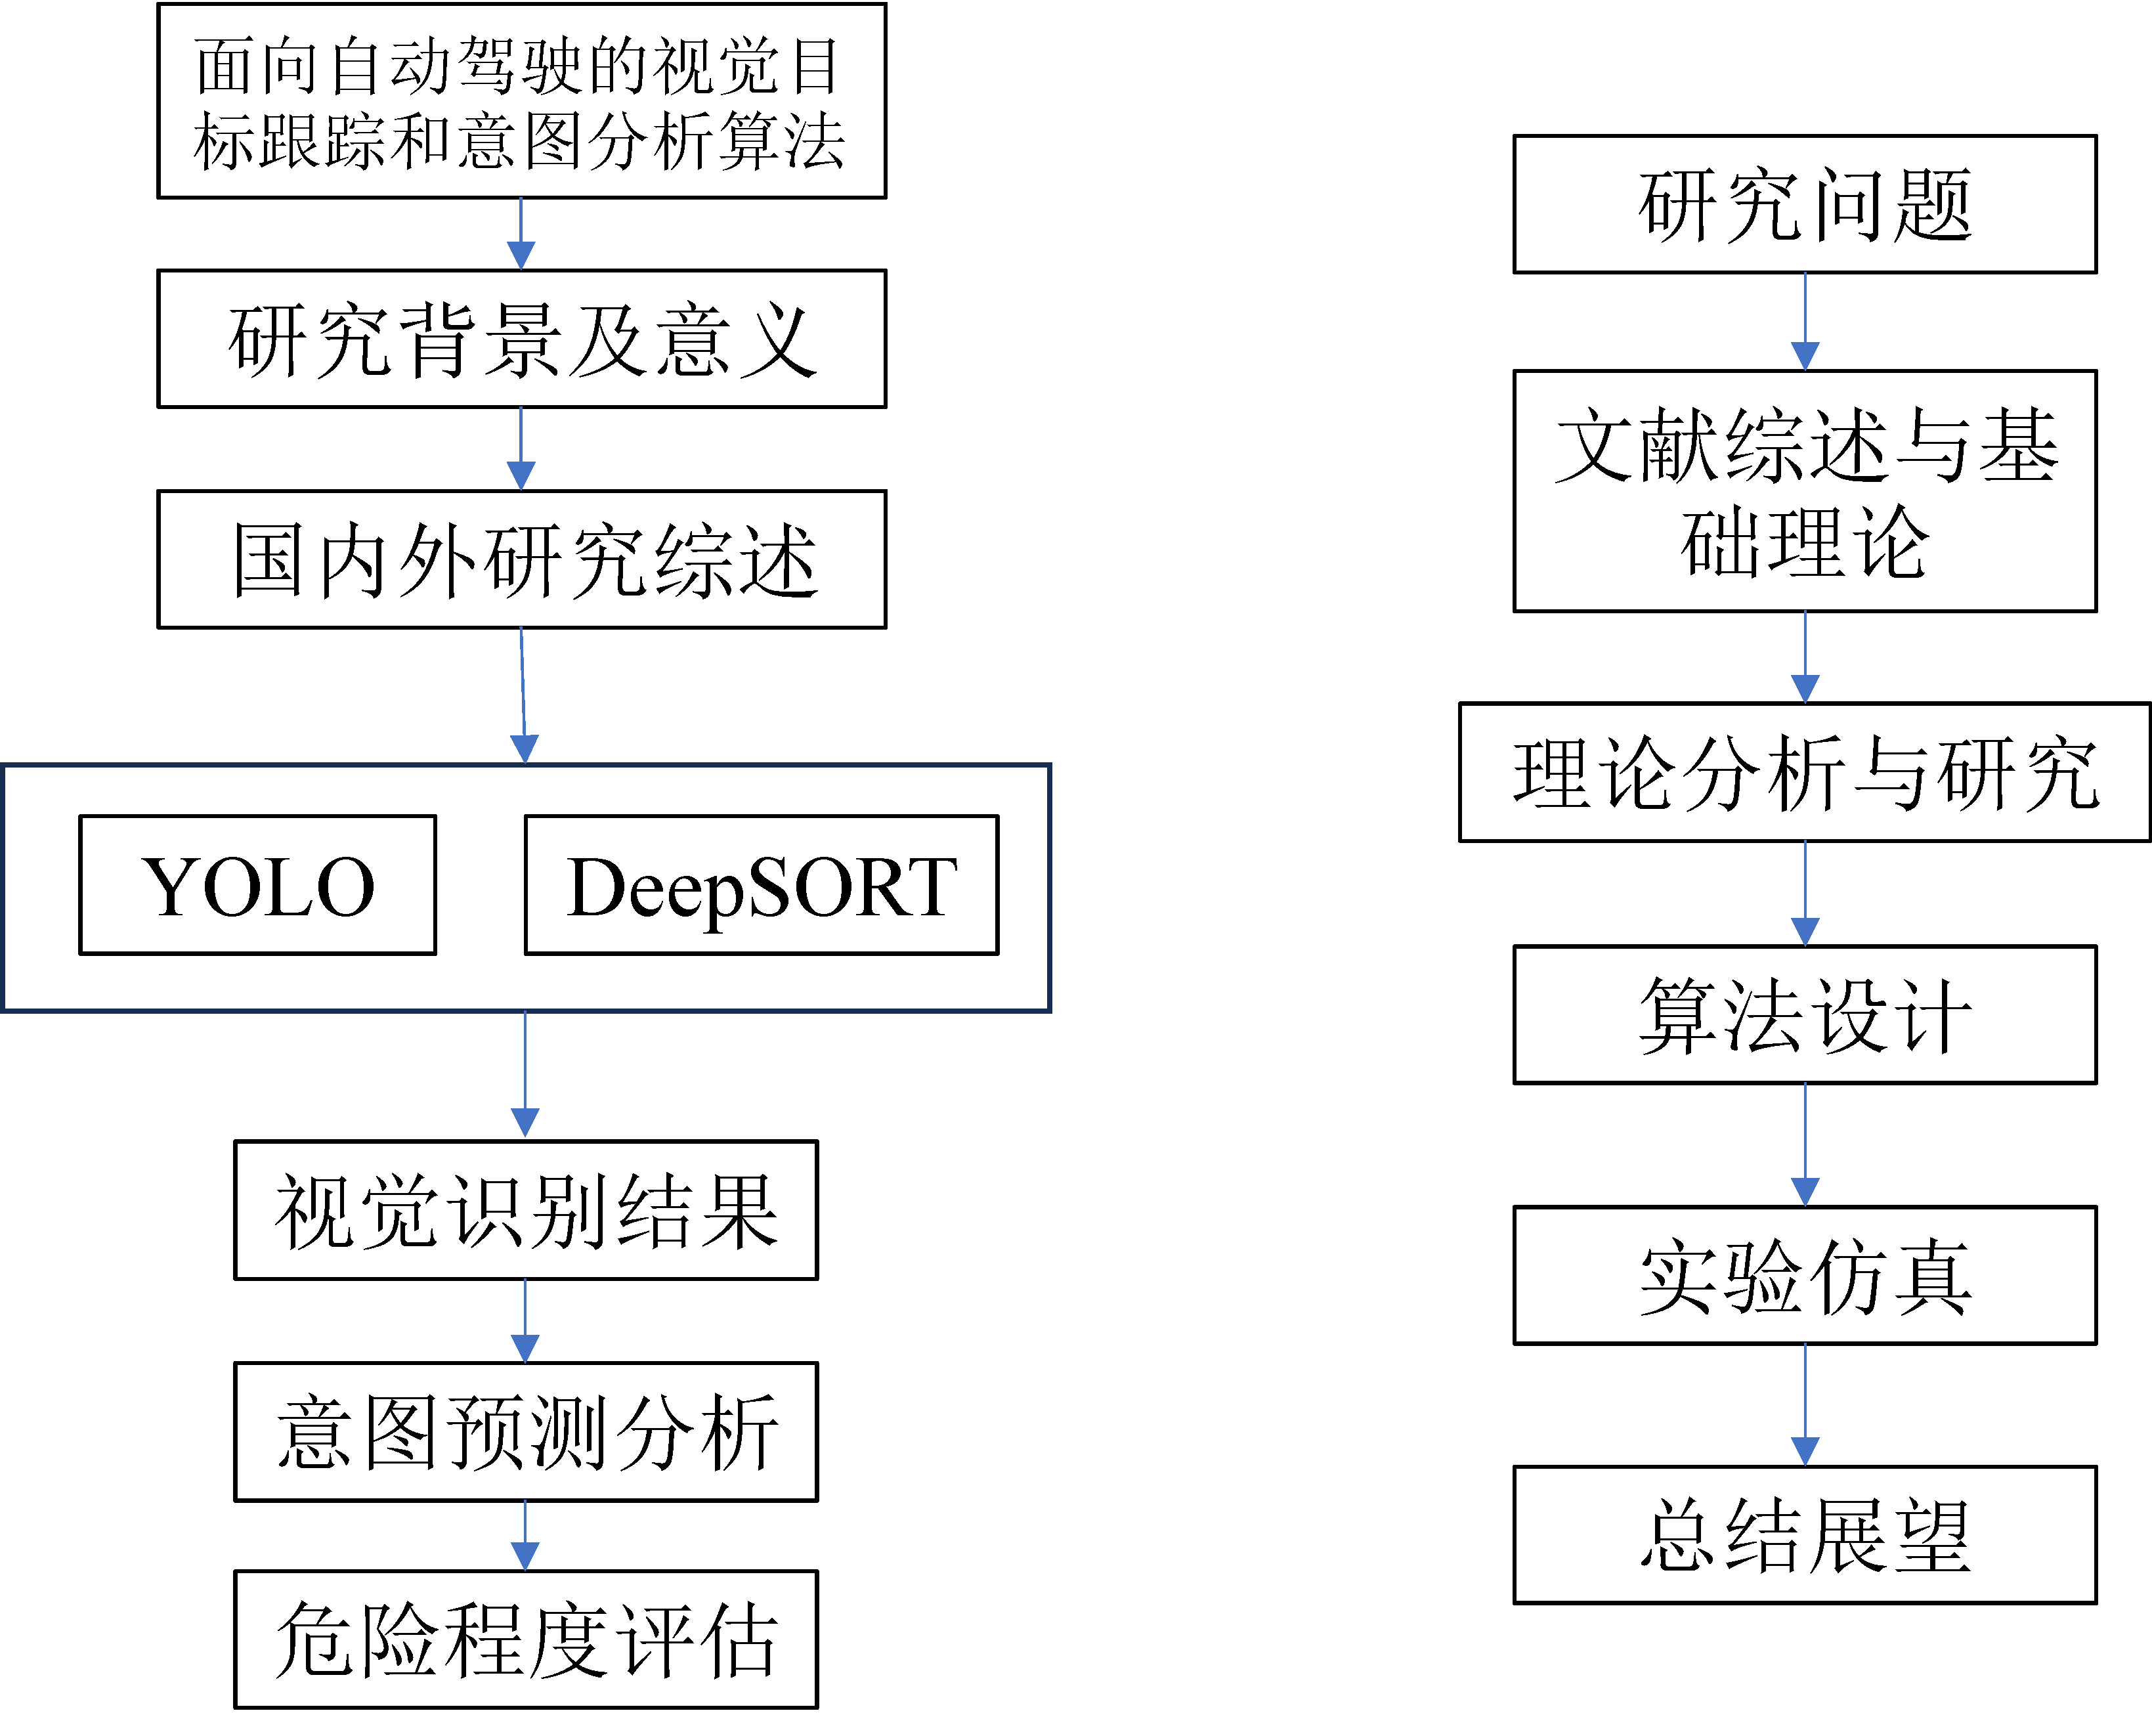
\includegraphics[width=0.8\textwidth]{images/p1_struct.pdf}  % 引用转换后的 PDF 文件
    \caption{图1 论文结构框架图}
    \label{fig:example_image}  % 可用于引用此图片
\end{figure}




\begin{tabular}{l l}
%  \verb|\songti| & {\songti 宋体} \\
%  \verb|\heiti| & {\heiti 黑体} \\
%   \verb|\kaiti| & {\kaiti 楷体}
\end{tabular}